\chapter{PENGUJIAN DAN ANALISIS}
\label{chap:pengujiananalisis}

% Ubah bagian-bagian berikut dengan isi dari pengujian dan analisis

Pada bab ini dipaparkan hasil pengujian serta analisa dari desain sistem dan implementasi. Pengujian dilakukan guna mengetahui tingkat kesalahan dan menarik kesimpulan dari sistem yang telah dibuat.

Pada proses pengujian digunakan salah satu layanan \textit{Google} yaitu \textit{Google Colaboratory} dengan spesifikasi \textit{hardware} seperti pada Tabel \ref{tab:spek-colab}. Sedangkan untuk spesifikasi \textit{hardware} komputer penulis dapat dilihat pada Tabel \ref{tab:spek-pc}.
\begin{table}[h]
	\begin{center}
		\caption{Spesifikasi \textit{hardware Google Colaboratory}}
		\begin{tabular}{ |c|c| } 
			\hline
			\textbf{Procesor} & Intel Xeon Processor @ 2.3 GHz\\
			\hline 
			\textbf{Graphic Card} & Tesla K80 12 GB GDDR5 VRAM\\
			\hline 
			\textbf{RAM} & 16 GB\\ 
			\hline
		\end{tabular}
		\label{tab:spek-colab}
	\end{center}
\end{table} 

\begin{table}[h]
	\begin{center}
		\caption{Spesifikasi \textit{hardware} Komputer yang Digunakan}
		\begin{tabular}{ |c|c| } 
			\hline
			\textbf{Procesor} & Intel(R) Core(TM) i5-10400F CPU @ 2.90GHz\\
			\hline 
			\textbf{Graphic Card} & Nvidia GeForce GTX 1650 4 GB GDDR6\\
			\hline 
			\textbf{RAM} & 8 GB\\ 
			\hline
		\end{tabular}
		\label{tab:spek-pc}
	\end{center}
\end{table}

Pengujian dilakukan dengan membagi model ke beberapa jenis \textit{backbone} yang digunakan, antara lain Resnet-50, Resnet-101, dan Mobilenet-V1.

\section{Pengujian Jenis \textit{Backbone}}
\label{sec:pengujian-backbone}

Pengujian pada jenis \textit{backbone} bertujuan untuk mengetahui performa dan akurasi dari setiap model yang dihasilkan dengan \textit{backbone} yang berbeda.

\subsection{Resnet-50}
\label{subsec:resnet50}

Tabel \ref{tab:conf-resnet50} merupakan parameter-parameter yang digunakan untuk membuat model Mask R-CNN dengan menggunakan \textit{backbone} Resnet-50.

% Please add the following required packages to your document preamble:
% \usepackage{longtable}
% Note: It may be necessary to compile the document several times to get a multi-page table to line up properly
\begin{longtable}[h]{|l|l|}
	\caption{Konfigurasi Model menggunakan Resnet-50}
	\label{tab:conf-resnet50}\\
	\hline
	\multicolumn{2}{|c|}{\textbf{Pengaturan Model Resnet-50}}                                                                                                                                                                \\ \hline
	\endfirsthead
	%
	\multicolumn{2}{c}%
	{{\tablename\ \thetable{} -- Lanjutan dari halaman sebelumnya}} \\
	\endhead
	%
	\multicolumn{2}{|r|}{\textit{Dilanjutkan pada halaman berikutnya}} \\ \hline
	\endfoot
	%
	\endlastfoot
	BACKBONE                        & resnet50                                                                                                                                                                               \\ \hline
	BACKBONE\_STRIDES               & {[}4, 8, 16, 32, 64{]}                                                                                                                                                                 \\ \hline
	BATCH\_SIZE                     & 1                                                                                                                                                                                      \\ \hline
	BBOX\_STD\_DEV                  & {[}0.1 0.1 0.2 0.2{]}                                                                                                                                                                  \\ \hline
	COMPUTE\_BACKBONE\_SHAPE        & None                                                                                                                                                                                   \\ \hline
	DETECTION\_MAX\_INSTANCES       & 50                                                                                                                                                                                     \\ \hline
	DETECTION\_MIN\_CONFIDENCE      & 0.9                                                                                                                                                                                    \\ \hline
	DETECTION\_NMS\_THRESHOLD       & 0.2                                                                                                                                                                                    \\ \hline
	FPN\_CLASSIF\_FC\_LAYERS\_SIZE  & 1024                                                                                                                                                                                   \\ \hline
	GPU\_COUNT                      & 1                                                                                                                                                                                      \\ \hline
	GRADIENT\_CLIP\_NORM            & 5.0                                                                                                                                                                                    \\ \hline
	IMAGES\_PER\_GPU                & 1                                                                                                                                                                                      \\ \hline
	IMAGE\_CHANNEL\_COUNT           & 3                                                                                                                                                                                      \\ \hline
	IMAGE\_MAX\_DIM                 & 512                                                                                                                                                                                    \\ \hline
	IMAGE\_META\_SIZE               & 16                                                                                                                                                                                     \\ \hline
	IMAGE\_MIN\_DIM                 & 400                                                                                                                                                                                    \\ \hline
	IMAGE\_MIN\_SCALE               & 0                                                                                                                                                                                      \\ \hline
	IMAGE\_RESIZE\_MODE             & square                                                                                                                                                                                 \\ \hline
	IMAGE\_SHAPE                    & {[}512 512 3{]}                                                                                                                                                                        \\ \hline
	LEARNING\_MOMENTUM              & 0.9                                                                                                                                                                                    \\ \hline
	LEARNING\_RATE                  & 0.001                                                                                                                                                                                  \\ \hline
	LOSS\_WEIGHTS                   & \begin{tabular}[c]{@{}l@{}}\{'rpn\_class\_loss': 1.0,\\  'rpn\_bbox\_loss': 1.0, \\ 'mrcnn\_class\_loss': 1.0, \\ 'mrcnn\_bbox\_loss': 1.0, \\ 'mrcnn\_mask\_loss': 1.0\}\end{tabular} \\ \hline
	MASK\_POOL\_SIZE                & 14                                                                                                                                                                                     \\ \hline
	MASK\_SHAPE                     & {[}28, 28{]}                                                                                                                                                                           \\ \hline
	MAX\_GT\_INSTANCES              & 50                                                                                                                                                                                     \\ \hline
	MEAN\_PIXEL                     & {[}123.7 116.8 103.9{]}                                                                                                                                                                \\ \hline
	MINI\_MASK\_SHAPE               & (56, 56)                                                                                                                                                                               \\ \hline
	NAME                            & object                                                                                                                                                                                 \\ \hline
	NUM\_CLASSES                    & 4                                                                                                                                                                                      \\ \hline
	POOL\_SIZE                      & 7                                                                                                                                                                                      \\ \hline
	POST\_NMS\_ROIS\_INFERENCE      & 1000                                                                                                                                                                                   \\ \hline
	POST\_NMS\_ROIS\_TRAINING       & 2000                                                                                                                                                                                   \\ \hline
	PRE\_NMS\_LIMIT                 & 6000                                                                                                                                                                                   \\ \hline
	ROI\_POSITIVE\_RATIO            & 0.33                                                                                                                                                                                   \\ \hline
	RPN\_ANCHOR\_RATIOS             & {[}0.5, 1, 2{]}                                                                                                                                                                        \\ \hline
	RPN\_ANCHOR\_SCALES             & (32, 64, 128, 256, 512)                                                                                                                                                                \\ \hline
	RPN\_ANCHOR\_STRIDE             & 1                                                                                                                                                                                      \\ \hline
	RPN\_BBOX\_STD\_DEV             & {[}0.1 0.1 0.2 0.2{]}                                                                                                                                                                  \\ \hline
	RPN\_NMS\_THRESHOLD             & 0.7                                                                                                                                                                                    \\ \hline
	RPN\_TRAIN\_ANCHORS\_PER\_IMAGE & 256                                                                                                                                                                                    \\ \hline
	STEPS\_PER\_EPOCH               & 100                                                                                                                                                                                    \\ \hline
	TOP\_DOWN\_PYRAMID\_SIZE        & 256                                                                                                                                                                                    \\ \hline
	TRAIN\_BN                       & False                                                                                                                                                                                  \\ \hline
	TRAIN\_ROIS\_PER\_IMAGE         & 200                                                                                                                                                                                    \\ \hline
	USE\_MINI\_MASK                 & True                                                                                                                                                                                   \\ \hline
	USE\_RPN\_ROIS                  & True                                                                                                                                                                                   \\ \hline
	VALIDATION\_STEPS               & 30                                                                                                                                                                                     \\ \hline
	WEIGHT\_DECAY                   & 0.0001
	\\ \hline                 
\end{longtable}

Setelah dilakukan serangkaian proses training yang memakan waktu sekitar 3 jam 40 menit 24 detik didapatkan \textit{output} berupa \textit{model file}  dengan format \textit{h5} yang mempunyai ukuran 170.9 MB. \textit{Training loss} terendah yang berhasil dicapai dengan menggunakan \textit{backbone} Resnet-50 (pada \textit{epoch} ke 242) adalah 0.4061 dengan rincian \textit{training bounding box loss} sebesar 0.04083, \textit{training classification loss} sebesar 0.02268 serta \textit{training mask loss} sebesar 0.139 (dimana $L=L_{bbox}+L_{cls}+L_{mask}$). Gambar \ref{fig:resnet50-training} merupakan grafik yang menunjukkan perubahan \textit{training loss, training bounding box loss, training classification loss,} serta \textit{training mask loss} dari \textit{epoch} 1 sampai 300.

\begin{figure}[H]
	\centering
	\begin{minipage}{0.45\textwidth}
		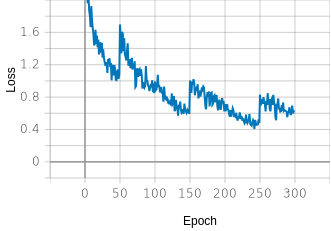
\includegraphics[width=\textwidth]{gambar/training_resnet50/tugas-akhir-Page-12.png}
		\caption*{(a) \textit{Training Loss}}
	\end{minipage}
	\hfill
	\begin{minipage}{0.45\textwidth}
		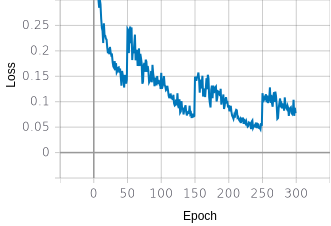
\includegraphics[width=\textwidth]{gambar/training_resnet50/tugas-akhir-Page-12-(1).png}
		\caption*{(b) \textit{Training Bounding Box Loss}}
	\end{minipage}
	\vfill
	\begin{minipage}{0.45\textwidth}
		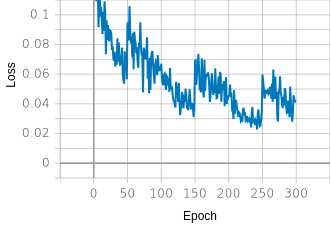
\includegraphics[width=\textwidth]{gambar/training_resnet50/tugas-akhir-Page-12-(2).png}
		\caption*{(c) \textit{Training Classification Loss}}
	\end{minipage}
	\hfill
	\begin{minipage}{0.45\textwidth}
		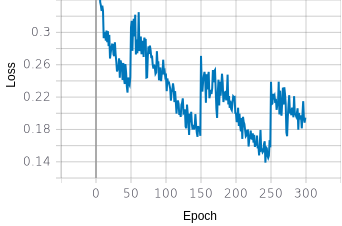
\includegraphics[width=\textwidth]{gambar/training_resnet50/tugas-akhir-Page-12-(3).png}
		\caption*{(d) \textit{Training Mask Loss}}
	\end{minipage}
	\caption{Grafik Perubahan \textit{Training Loss} pada \textit{Resnet-50}}
	\label{fig:resnet50-training}
\end{figure}

Sedangkan pada saat proses \textit{validation} sendiri \textit{Loss} terendah yang berhasil dicapai pada \textit{epoch} ke 266 dengan nilai sebesar 0.3653 dengan rincian \textit{validation bounding box loss} sebesar 0.4556, \textit{validation classification loss} sebesar 0.01912 serta \textit{validation mask loss} sebesar 0.1519. Namun untuk \textit{validation bounding box loss} terendah berada pada \textit{epoch} ke 260 dengan nilai sebesar 0.4203 sedangkan \textit{validation classification loss} terendah pada \textit{epoch} ke 210 dengan nilai 0.01525 serta \textit{validation mask loss} terendah pada \textit{epoch} ke 201 dengan nilai 0.1439. Gambar \ref{fig:resnet50-val} merupakan grafik yang menunjukkan perubahan \textit{validation loss, validation bounding box loss, validation classification loss,} serta \textit{validation mask loss} dari \textit{epoch} 1 sampai 300.

\begin{figure}[H]
	\centering
	\begin{minipage}{0.45\textwidth}
		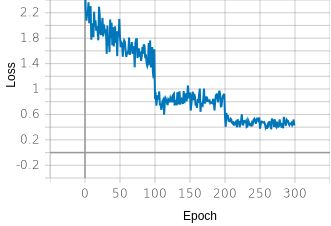
\includegraphics[width=\textwidth]{gambar/training_resnet50/tugas-akhir-Page-13.png}
		\caption*{(a) \textit{Validation Loss}}
	\end{minipage}
	\hfill
	\begin{minipage}{0.45\textwidth}
		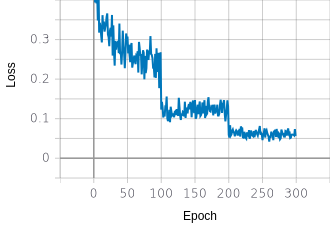
\includegraphics[width=\textwidth]{gambar/training_resnet50/tugas-akhir-Page-13 (1).png}
		\caption*{(b) \textit{Validation Bounding Box Loss}}
	\end{minipage}
	\vfill
	\begin{minipage}{0.45\textwidth}
		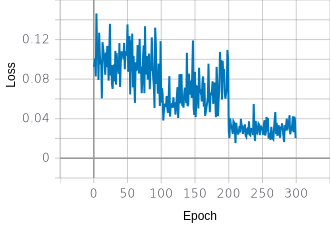
\includegraphics[width=\textwidth]{gambar/training_resnet50/tugas-akhir-Page-13 (2).png}
		\caption*{(c) \textit{Validation Classification Loss}}
	\end{minipage}
	\hfill
	\begin{minipage}{0.45\textwidth}
		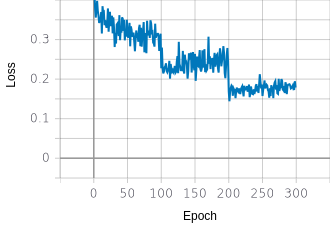
\includegraphics[width=\textwidth]{gambar/training_resnet50/tugas-akhir-Page-13 (3).png}
		\caption*{(d) \textit{Validation Mask Loss}}
	\end{minipage}
	\caption{Grafik Perubahan \textit{Validation Loss} pada \textit{Resnet-50}}
	\label{fig:resnet50-val}
\end{figure}

Selain menggunakan \textit{Loss Function} untuk mengukur peforma hasil \textit{training} yang sudah dilakukan, digunakan juga \textit{mean Average Precision (mAP)}. \textit{Precision} sendiri merupakan fungsi untuk menggambarkan tingkat keakuratan antara data yang diminta dengan hasil prediksi yang diberikan oleh model. Maka, \textit{precision} merupakan rasio prediksi benar positif (TP) dibandingkan dengan keseluruhan hasil yang diprediksi positif (TP dan FP). Rumus untuk mencari \textit{Precision} adalah sebagai berikut :
\begin{equation}
	Precision = \frac{TP}{TP+FP} 
\end{equation}

Perhitungan \textit{mAP} pada penelitian ini dilakukan setiap 5 \textit{epoch} sekali, karena jika dilakukan setiap \textit{epoch} akan memerlukan \textit{training time} yang lebih lama serta \textit{resource hardware} yang diperlukan lebih besar. Nilai \textit{mAP} tertinggi didapatkan pada \textit{epoch} ke 220 sebesar 94.92. Gambar \ref{fig:resnet50-map} merupakan grafik yang menunjukan perubahan \textit{validation mean Average Precision} dari \textit{epoch} 1 sampai 300. 

\begin{figure}[h]
	\centering
	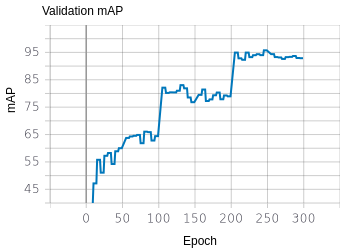
\includegraphics[scale=0.4]{gambar/resnet50-map.png}
	\caption{Grafik Perubahan \textit{Validation mAP} pada Resnet-50}
	\label{fig:resnet50-map}
\end{figure}

\newpage

\subsection{Resnet-101}
\label{subsec:resnet101}

Tabel \ref{tab:conf-resnet101} merupakan parameter-parameter yang digunakan untuk membuat model Mask R-CNN dengan menggunakan \textit{backbone} Resnet-101.

% Please add the following required packages to your document preamble:
% \usepackage{longtable}
% Note: It may be necessary to compile the document several times to get a multi-page table to line up properly
\begin{longtable}{|l|l|}
	\caption{Konfigurasi Model menggunakan Resnet-101}
	\label{tab:conf-resnet101}\\
	\hline
	\multicolumn{2}{|c|}{\textbf{Pengaturan Model Resnet-101}}                                                                                                                                                             \\ \hline
	\endfirsthead
	%
	\multicolumn{2}{c}%
	{{\tablename\ \thetable{} -- Lanjutan dari halaman sebelumnya}} \\
	\endhead
	%
	\multicolumn{2}{|r|}{\textit{Dilanjutkan pada halaman berikutnya}} \\ \hline
	\endfoot
	%
	\endlastfoot
	BACKBONE                        & resnet101                                                                                                                                                                            \\ \hline
	BACKBONE\_STRIDES               & {[}4, 8, 16, 32, 64{]}                                                                                                                                                                 \\ \hline
	BATCH\_SIZE                     & 1                                                                                                                                                                                      \\ \hline
	BBOX\_STD\_DEV                  & {[}0.1 0.1 0.2 0.2{]}                                                                                                                                                                  \\ \hline
	COMPUTE\_BACKBONE\_SHAPE        & None                                                                                                                                                                                   \\ \hline
	DETECTION\_MAX\_INSTANCES       & 50                                                                                                                                                                                     \\ \hline
	DETECTION\_MIN\_CONFIDENCE      & 0.9                                                                                                                                                                                    \\ \hline
	DETECTION\_NMS\_THRESHOLD       & 0.2                                                                                                                                                                                    \\ \hline
	FPN\_CLASSIF\_FC\_LAYERS\_SIZE  & 1024                                                                                                                                                                                   \\ \hline
	GPU\_COUNT                      & 1                                                                                                                                                                                      \\ \hline
	GRADIENT\_CLIP\_NORM            & 5.0                                                                                                                                                                                    \\ \hline
	IMAGES\_PER\_GPU                & 1                                                                                                                                                                                      \\ \hline
	IMAGE\_CHANNEL\_COUNT           & 3                                                                                                                                                                                      \\ \hline
	IMAGE\_MAX\_DIM                 & 512                                                                                                                                                                                    \\ \hline
	IMAGE\_META\_SIZE               & 16                                                                                                                                                                                     \\ \hline
	IMAGE\_MIN\_DIM                 & 400                                                                                                                                                                                    \\ \hline
	IMAGE\_MIN\_SCALE               & 0                                                                                                                                                                                      \\ \hline
	IMAGE\_RESIZE\_MODE             & square                                                                                                                                                                                 \\ \hline
	IMAGE\_SHAPE                    & {[}512 512 3{]}                                                                                                                                                                        \\ \hline
	LEARNING\_MOMENTUM              & 0.9                                                                                                                                                                                    \\ \hline
	LEARNING\_RATE                  & 0.001                                                                                                                                                                                  \\ \hline
	LOSS\_WEIGHTS                   & \begin{tabular}[c]{@{}l@{}}\{'rpn\_class\_loss': 1.0,\\  'rpn\_bbox\_loss': 1.0, \\ 'mrcnn\_class\_loss': 1.0, \\ 'mrcnn\_bbox\_loss': 1.0, \\ 'mrcnn\_mask\_loss': 1.0\}\end{tabular} \\ \hline
	MASK\_POOL\_SIZE                & 14                                                                                                                                                                                     \\ \hline
	MASK\_SHAPE                     & {[}28, 28{]}                                                                                                                                                                           \\ \hline
	MAX\_GT\_INSTANCES              & 50                                                                                                                                                                                     \\ \hline
	MEAN\_PIXEL                     & {[}123.7 116.8 103.9{]}                                                                                                                                                                \\ \hline
	MINI\_MASK\_SHAPE               & (56, 56)                                                                                                                                                                               \\ \hline
	NAME                            & object                                                                                                                                                                                 \\ \hline
	NUM\_CLASSES                    & 4                                                                                                                                                                                      \\ \hline
	POOL\_SIZE                      & 7                                                                                                                                                                                      \\ \hline
	POST\_NMS\_ROIS\_INFERENCE      & 1000                                                                                                                                                                                   \\ \hline
	POST\_NMS\_ROIS\_TRAINING       & 2000                                                                                                                                                                                   \\ \hline
	PRE\_NMS\_LIMIT                 & 6000                                                                                                                                                                                   \\ \hline
	ROI\_POSITIVE\_RATIO            & 0.33                                                                                                                                                                                   \\ \hline
	RPN\_ANCHOR\_RATIOS             & {[}0.5, 1, 2{]}                                                                                                                                                                        \\ \hline
	RPN\_ANCHOR\_SCALES             & (32, 64, 128, 256, 512)                                                                                                                                                                \\ \hline
	RPN\_ANCHOR\_STRIDE             & 1                                                                                                                                                                                      \\ \hline
	RPN\_BBOX\_STD\_DEV             & {[}0.1 0.1 0.2 0.2{]}                                                                                                                                                                  \\ \hline
	RPN\_NMS\_THRESHOLD             & 0.7                                                                                                                                                                                    \\ \hline
	RPN\_TRAIN\_ANCHORS\_PER\_IMAGE & 256                                                                                                                                                                                    \\ \hline
	STEPS\_PER\_EPOCH               & 100                                                                                                                                                                                    \\ \hline
	TOP\_DOWN\_PYRAMID\_SIZE        & 256                                                                                                                                                                                    \\ \hline
	TRAIN\_BN                       & False                                                                                                                                                                                  \\ \hline
	TRAIN\_ROIS\_PER\_IMAGE         & 200                                                                                                                                                                                    \\ \hline
	USE\_MINI\_MASK                 & True                                                                                                                                                                                   \\ \hline
	USE\_RPN\_ROIS                  & True                                                                                                                                                                                   \\ \hline
	VALIDATION\_STEPS               & 30                                                                                                                                                                                     \\ \hline
	WEIGHT\_DECAY                   & 0.0001                                                                                                                                                                                 \\ \hline
\end{longtable}

Setelah dilakukan serangkaian proses training yang memakan waktu sekitar 4 jam 9 menit 16 detik didapatkan \textit{output} berupa \textit{model file}  dengan format \textit{h5} yang mempunyai ukuran 244 MB. \textit{Training loss} terendah yang berhasil dicapai dengan menggunakan \textit{backbone} Resnet-101 (pada \textit{epoch} ke 244) adalah 0.3933 dengan rincian \textit{training bounding box loss} sebesar 0.04164, \textit{training classification loss} sebesar 0.0247 serta \textit{training mask loss} sebesar 0.1403. Namun untuk \textit{training bounding box loss} terendah terdapat pada \textit{epoch} ke 246 dengan nilai sebesar 0.04083, \textit{training classification loss} terendah pada \textit{epoch} ke 234 dengan nilai 0.01957. Gambar \ref{fig:resnet101-training} merupakan grafik yang menunjukkan perubahan \textit{training loss, training bounding box loss, training classification loss,} serta \textit{training mask loss} dari \textit{epoch} 1 sampai 300. 

\begin{figure}[H]
	\centering
	\begin{minipage}{0.45\textwidth}
		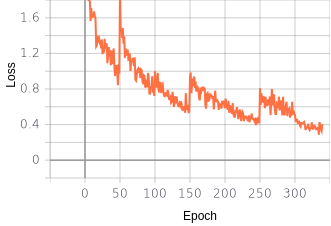
\includegraphics[width=\textwidth]{gambar/training_resnet50/tugas-akhir-Page-15.png}
		\caption*{(a) \textit{Training Loss}}
	\end{minipage}
	\hfill
	\begin{minipage}{0.45\textwidth}
		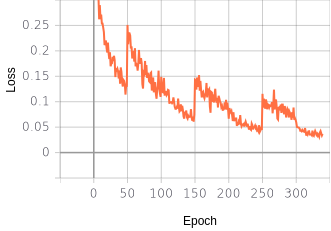
\includegraphics[width=\textwidth]{gambar/training_resnet50/tugas-akhir-Page-15 (1).png}
		\caption*{(b) \textit{Training Bounding Box Loss}}
	\end{minipage}
	\vfill
	\begin{minipage}{0.45\textwidth}
		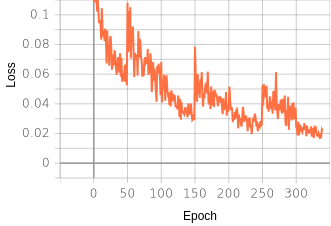
\includegraphics[width=\textwidth]{gambar/training_resnet50/tugas-akhir-Page-15 (2).png}
		\caption*{(c) \textit{Training Classification Loss}}
	\end{minipage}
	\hfill
	\begin{minipage}{0.45\textwidth}
		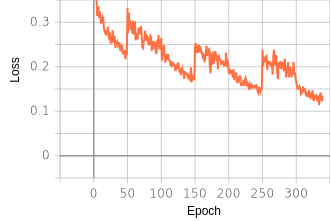
\includegraphics[width=\textwidth]{gambar/training_resnet50/tugas-akhir-Page-15 (3).png}
		\caption*{(d) \textit{Training Mask Loss}}
	\end{minipage}
	\caption{Grafik Perubahan \textit{Training Loss} pada \textit{Resnet-101}}
	\label{fig:resnet101-training}
\end{figure}

Sedangkan pada saat proses \textit{validation} sendiri \textit{Loss} terendah yang berhasil dicapai pada \textit{epoch} ke 266 dengan nilai sebesar 0.299 dengan rincian \textit{validation bounding box loss} sebesar 0.03867, \textit{validation classification loss} sebesar 0.01246 serta \textit{validation mask loss} sebesar 0.1461. Gambar \ref{fig:resnet101-val} merupakan grafik yang menunjukkan perubahan \textit{validation loss, validation bounding box loss, validation classification loss,} serta \textit{validation mask loss} dari \textit{epoch} 1 sampai 300.

\begin{figure}[H]
	\centering
	\begin{minipage}{0.45\textwidth}
		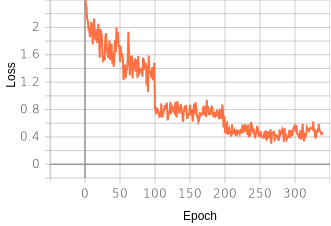
\includegraphics[width=\textwidth]{gambar/training_resnet50/tugas-akhir-Page-16.png}
		\caption*{(a) \textit{Validation Loss}}
	\end{minipage}
	\hfill
	\begin{minipage}{0.45\textwidth}
		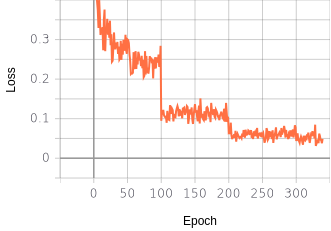
\includegraphics[width=\textwidth]{gambar/training_resnet50/tugas-akhir-Page-16 (1).png}
		\caption*{(b) \textit{Validation Bounding Box Loss}}
	\end{minipage}
	\vfill
	\begin{minipage}{0.45\textwidth}
		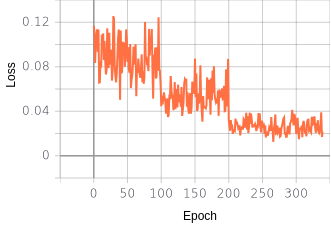
\includegraphics[width=\textwidth]{gambar/training_resnet50/tugas-akhir-Page-16 (2).png}
		\caption*{(c) \textit{Validation Classification Loss}}
	\end{minipage}
	\hfill
	\begin{minipage}{0.45\textwidth}
		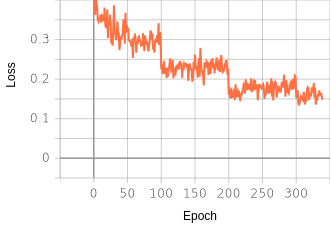
\includegraphics[width=\textwidth]{gambar/training_resnet50/tugas-akhir-Page-16 (3).png}
		\caption*{(d) \textit{Validation Mask Loss}}
	\end{minipage}
	\caption{Grafik Perubahan \textit{Validation Loss} pada \textit{Resnet-101}}
	\label{fig:resnet101-val}
\end{figure}

Nilai \textit{mAP} tertinggi didapatkan pada \textit{epoch} ke 215 sebesar 96.21. Gambar \ref{fig:resnet101-map} merupakan grafik yang menunjukan perubahan \textit{validation mean Average Precision} dari \textit{epoch} 1 sampai 300.

\begin{figure}[h]
	\centering
	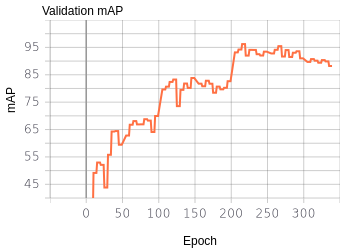
\includegraphics[scale=0.4]{gambar/resnet101-map.png}
	\caption{Grafik Perubahan \textit{Validation mAP} pada \textit{Resnet-101}}
	\label{fig:resnet101-map}
\end{figure} 

\newpage

\subsection{MobileNet-V1}
\label{subsec:mobilenetv1}

Tabel \ref{tab:conf-mobilenet-v1} merupakan parameter-parameter yang digunakan untuk membuat model Mask R-CNN dengan menggunakan \textit{backbone} Mobilenet-V1.

% Please add the following required packages to your document preamble:
% \usepackage{longtable}
% Note: It may be necessary to compile the document several times to get a multi-page table to line up properly
\begin{longtable}[h]{|l|l|}
	\caption{Konfigurasi Model menggunakan Mobilenet-V1}
	\label{tab:conf-mobilenet-v1}\\
	\hline
	\multicolumn{2}{|c|}{\textbf{Pengaturan Model Mobilenet-V1}}                                                                                                                                                             
	\\ \hline
	\endfirsthead
	%
	\multicolumn{2}{c}%
	{{\tablename\ \thetable{} -- Lanjutan dari halaman sebelumnya}} \\
	\endhead
	%
	\multicolumn{2}{|r|}{\textit{Dilanjutkan pada halaman berikutnya}} \\ \hline
	\endfoot
	%
	\endlastfoot
	BACKBONE                        & mobilenetv1                                                                                                                                                                            \\ \hline
	BACKBONE\_STRIDES               & {[}4, 8, 16, 32, 64{]}                                                                                                                                                                 \\ \hline
	BATCH\_SIZE                     & 1                                                                                                                                                                                      \\ \hline
	BBOX\_STD\_DEV                  & {[}0.1 0.1 0.2 0.2{]}                                                                                                                                                                  \\ \hline
	COMPUTE\_BACKBONE\_SHAPE        & None                                                                                                                                                                                   \\ \hline
	DETECTION\_MAX\_INSTANCES       & 50                                                                                                                                                                                     \\ \hline
	DETECTION\_MIN\_CONFIDENCE      & 0.9                                                                                                                                                                                    \\ \hline
	DETECTION\_NMS\_THRESHOLD       & 0.2                                                                                                                                                                                    \\ \hline
	FPN\_CLASSIF\_FC\_LAYERS\_SIZE  & 1024                                                                                                                                                                                   \\ \hline
	GPU\_COUNT                      & 1                                                                                                                                                                                      \\ \hline
	GRADIENT\_CLIP\_NORM            & 5.0                                                                                                                                                                                    \\ \hline
	IMAGES\_PER\_GPU                & 1                                                                                                                                                                                      \\ \hline
	IMAGE\_CHANNEL\_COUNT           & 3                                                                                                                                                                                      \\ \hline
	IMAGE\_MAX\_DIM                 & 512                                                                                                                                                                                    \\ \hline
	IMAGE\_META\_SIZE               & 16                                                                                                                                                                                     \\ \hline
	IMAGE\_MIN\_DIM                 & 400                                                                                                                                                                                    \\ \hline
	IMAGE\_MIN\_SCALE               & 0                                                                                                                                                                                      \\ \hline
	IMAGE\_RESIZE\_MODE             & square                                                                                                                                                                                 \\ \hline
	IMAGE\_SHAPE                    & {[}512 512 3{]}                                                                                                                                                                        \\ \hline
	LEARNING\_MOMENTUM              & 0.9                                                                                                                                                                                    \\ \hline
	LEARNING\_RATE                  & 0.001                                                                                                                                                                                  \\ \hline
	LOSS\_WEIGHTS                   & \begin{tabular}[c]{@{}l@{}}\{'rpn\_class\_loss': 1.0,\\  'rpn\_bbox\_loss': 1.0, \\ 'mrcnn\_class\_loss': 1.0, \\ 'mrcnn\_bbox\_loss': 1.0, \\ 'mrcnn\_mask\_loss': 1.0\}\end{tabular} \\ \hline
	MASK\_POOL\_SIZE                & 14                                                                                                                                                                                     \\ \hline
	MASK\_SHAPE                     & {[}28, 28{]}                                                                                                                                                                           \\ \hline
	MAX\_GT\_INSTANCES              & 50                                                                                                                                                                                     \\ \hline
	MEAN\_PIXEL                     & {[}123.7 116.8 103.9{]}                                                                                                                                                                \\ \hline
	MINI\_MASK\_SHAPE               & (56, 56)                                                                                                                                                                               \\ \hline
	NAME                            & object                                                                                                                                                                                 \\ \hline
	NUM\_CLASSES                    & 4                                                                                                                                                                                      \\ \hline
	POOL\_SIZE                      & 7                                                                                                                                                                                      \\ \hline
	POST\_NMS\_ROIS\_INFERENCE      & 1000                                                                                                                                                                                   \\ \hline
	POST\_NMS\_ROIS\_TRAINING       & 2000                                                                                                                                                                                   \\ \hline
	PRE\_NMS\_LIMIT                 & 6000                                                                                                                                                                                   \\ \hline
	ROI\_POSITIVE\_RATIO            & 0.33                                                                                                                                                                                   \\ \hline
	RPN\_ANCHOR\_RATIOS             & {[}0.5, 1, 2{]}                                                                                                                                                                        \\ \hline
	RPN\_ANCHOR\_SCALES             & (32, 64, 128, 256, 512)                                                                                                                                                                \\ \hline
	RPN\_ANCHOR\_STRIDE             & 1                                                                                                                                                                                      \\ \hline
	RPN\_BBOX\_STD\_DEV             & {[}0.1 0.1 0.2 0.2{]}                                                                                                                                                                  \\ \hline
	RPN\_NMS\_THRESHOLD             & 0.7                                                                                                                                                                                    \\ \hline
	RPN\_TRAIN\_ANCHORS\_PER\_IMAGE & 256                                                                                                                                                                                    \\ \hline
	STEPS\_PER\_EPOCH               & 100                                                                                                                                                                                    \\ \hline
	TOP\_DOWN\_PYRAMID\_SIZE        & 256                                                                                                                                                                                    \\ \hline
	TRAIN\_BN                       & False                                                                                                                                                                                  \\ \hline
	TRAIN\_ROIS\_PER\_IMAGE         & 200                                                                                                                                                                                    \\ \hline
	USE\_MINI\_MASK                 & True                                                                                                                                                                                   \\ \hline
	USE\_RPN\_ROIS                  & True                                                                                                                                                                                   \\ \hline
	VALIDATION\_STEPS               & 30                                                                                                                                                                                     \\ \hline
	WEIGHT\_DECAY                   & 0.0001                                                                                                                                                                                 \\ \hline
\end{longtable}

Setelah dilakukan serangkaian proses training yang memakan waktu sekitar 3 jam 18 menit 44 detik didapatkan \textit{output} berupa \textit{model file}  dengan format \textit{h5} yang mempunyai ukuran 83.3 MB. \textit{Training loss} terendah yang berhasil dicapai dengan menggunakan \textit{backbone} Mobilenet-V1 (pada \textit{epoch} ke 46) adalah 1.604 dengan rincian \textit{training bounding box loss} sebesar 0.2322, \textit{training classification loss} sebesar 0.07858 serta \textit{training mask loss} sebesar 0.6729. Namun untuk \textit{training bounding box loss} terendah terdapat pada \textit{epoch} ke 48 dengan nilai sebesar 0.2239, \textit{training classification loss} terendah pada \textit{epoch} ke 61 dengan nilai 0.06219 serta \textit{training mask loss} terendah pada \textit{epoch} ke 61 sebesar 0.5701. Gambar \ref{fig:mobilenet-training} merupakan grafik yang menunjukkan perubahan \textit{training loss, training bounding box loss, training classification loss,} serta \textit{training mask loss} dari \textit{epoch} 1 sampai 300. 

\begin{figure}[H]
	\centering
	\begin{minipage}{0.45\textwidth}
		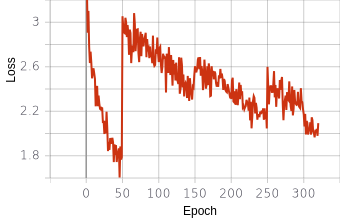
\includegraphics[width=\textwidth]{gambar/training_resnet50/tugas-akhir-Page 18.png}
		\caption*{(a) \textit{Training Loss}}
	\end{minipage}
	\hfill
	\begin{minipage}{0.45\textwidth}
		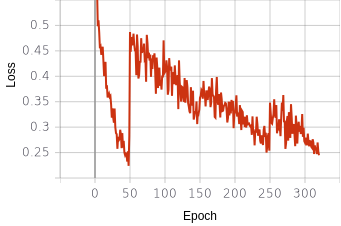
\includegraphics[width=\textwidth]{gambar/training_resnet50/tugas-akhir-Page 18 (1).png}
		\caption*{(b) \textit{Training Bounding Box Loss}}
	\end{minipage}
	\vfill
	\begin{minipage}{0.45\textwidth}
		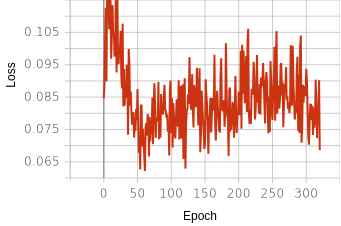
\includegraphics[width=\textwidth]{gambar/training_resnet50/tugas-akhir-Page 18 (2).png}
		\caption*{(c) \textit{Training Classification Loss}}
	\end{minipage}
	\hfill
	\begin{minipage}{0.45\textwidth}
		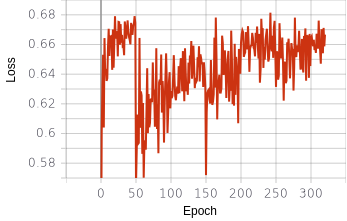
\includegraphics[width=\textwidth]{gambar/training_resnet50/tugas-akhir-Page 18 (3).png}
		\caption*{(d) \textit{Training Mask Loss}}
	\end{minipage}
	\caption{Grafik Perubahan \textit{Training Loss} pada \textit{MobileNet-V1}}
	\label{fig:mobilenetv1-training}
\end{figure}


Sedangkan pada saat proses \textit{validation} sendiri \textit{Loss} terendah yang berhasil dicapai pada \textit{epoch} ke 281 dengan nilai sebesar 1.624 dengan rincian \textit{validation bounding box loss} sebesar 0.2088, \textit{validation classification loss} sebesar 0.04799 serta \textit{validation mask loss} sebesar 0.6001. Namun untuk \textit{validation bounding box loss} terendah berada pada \textit{epoch} ke 300 dengan nilai sebesar 0.1927 sedangkan \textit{validation classification loss} terendah pada \textit{epoch} ke 70 dengan nilai 0.02607 serta \textit{validation mask loss} terendah pada \textit{epoch} ke 295 dengan nilai 0.5625. Gambar \ref{fig:mobilenetv1-val} merupakan grafik yang menunjukkan perubahan \textit{validation loss, validation bounding box loss, validation classification loss,} serta \textit{validation mask loss} dari \textit{epoch} 1 sampai 300.

\begin{figure}[H]
	\centering
	\begin{minipage}{0.45\textwidth}
		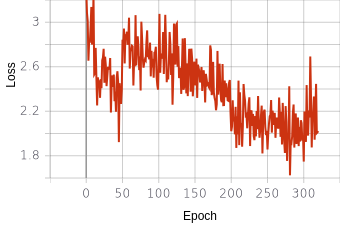
\includegraphics[width=\textwidth]{gambar/training_resnet50/tugas-akhir-Page 19.png}
		\caption*{(a) \textit{Validation Loss}}
	\end{minipage}
	\hfill
	\begin{minipage}{0.45\textwidth}
		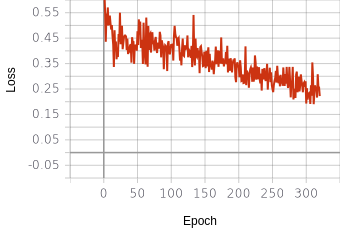
\includegraphics[width=\textwidth]{gambar/training_resnet50/tugas-akhir-Page 19 (1).png}
		\caption*{(b) \textit{Validation Bounding Box Loss}}
	\end{minipage}
	\vfill
	\begin{minipage}{0.45\textwidth}
		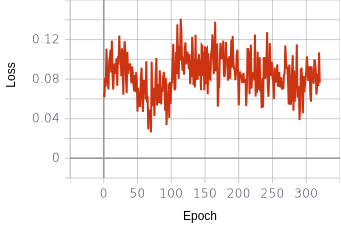
\includegraphics[width=\textwidth]{gambar/training_resnet50/tugas-akhir-Page 19 (2).png}
		\caption*{(c) \textit{Validation Classification Loss}}
	\end{minipage}
	\hfill
	\begin{minipage}{0.45\textwidth}
		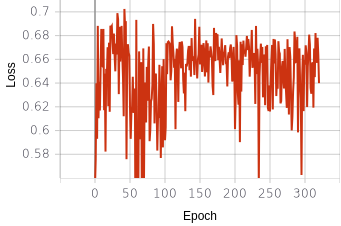
\includegraphics[width=\textwidth]{gambar/training_resnet50/tugas-akhir-Page 19 (3).png}
		\caption*{(d) \textit{Validation Mask Loss}}
	\end{minipage}
	\caption{Grafik Perubahan \textit{Validation Loss} pada \textit{MobileNet-V1}}
	\label{fig:mobilenetv1-val}
\end{figure}

Nilai \textit{mAP} tertinggi didapatkan pada \textit{epoch} ke 210 sebesar 26.04. Gambar \ref{fig:mobilenetv1-map} merupakan grafik yang menunjukan perubahan \textit{validation mean Average Precision} dari \textit{epoch} 1 sampai 300.

\newpage

\begin{figure}[h]
	\centering
	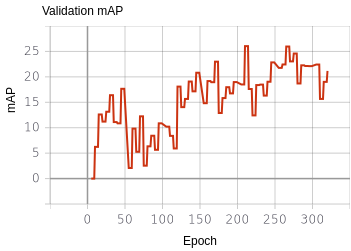
\includegraphics[scale=0.4]{gambar/mobilenetv1-map.png}
	\caption{Grafik Perubahan \textit{Validation mAP} pada \textit{MobileNet-V1}}
	\label{fig:mobilenetv1-map}
\end{figure} 

Tabel \ref{tab:train-recap} adalah tabel perbandingan dari \textit{output file size} dan \textit{mAP} dari total 3 model dengan \textit{backbone} berbeda yang diuji. Tahap ini masih merupakan hasil tahap \textit{training}. Sedangkan Gambar \ref{fig:graph-recap} merupakan grafik perbandingan \textit{mAP} dengan \textit{file size}. Proses selanjutnya setelah mendapatkan hasil yang ditunjukkan pada setiap model adalah melakukan proses prediksi atau melakukan \textit{testing data}.

\begin{table}[h]
	\centering
	\caption{Tabel Perbandingan Model dengan \textit{backbone} yang berbeda}
	\begin{tabular}{|c|l|l|l|}
		\hline
		\textbf{No.} & \multicolumn{1}{c|}{\textit{\textbf{Backbone}}} & \multicolumn{1}{c|}{\textit{\textbf{Output File Size}}} & \multicolumn{1}{c|}{\textbf{mAP}} \\ \hline
		1            & Resnet-50                                       & 170.9 MB                                                & 94.92\%                           \\ \hline
		2            & Resnet-101                                      & 244 MB                                                  & 96.21\%                           \\ \hline
		3            & Mobilenet-V1                                    & 83.3 MB                                                 & 26.04\%                           \\ \hline
	\end{tabular}
	\label{tab:train-recap}
\end{table}

\newpage

\begin{figure}[h]
	\centering
	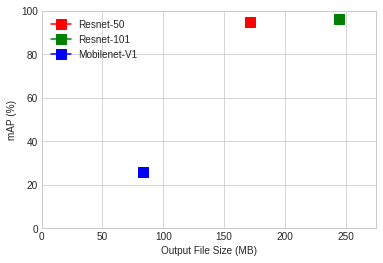
\includegraphics[scale=0.75]{gambar/graph-recap.png}
	\caption{Grafik Perbandingan Model dengan \textit{backbone} yang berbeda}
	\label{fig:graph-recap}
\end{figure}

\subsection{Perbandingan Hasil Prediksi}
\label{subsec:perbandingan-hasil-prediksi}

Setelah mendapatkan hasil \textit{training} pada Tabel \ref{tab:train-recap} terdapat dua parameter yang digunakan yaitu \textit{output file size} dan \textit{mean Average Precision}. Parameter tersebut digunakan untuk melakukan justifikasi dalam pemilihan model yang terbaik. Pada parameter \textit{output file size}, model yang diinginkan adalah model dengan dengan ukuran sekecil mungkin, agar tidak menghabiskan kapasitas penyimpanan terlalu banyak. Sedangkan untuk \textit{mean Average Precision} yang diinginkan adalah model dengan \textit{meand Average Precision} yang tinggi sehingga kemam puan model tersebut untuk melakukan proses prediksi akan semakin tepat dengan kondisi yang sesuai pada dunia nyata.

Setelah membandingkan parameter \textit{output file size} dan \textit{mean Average Precision}, pada tahap selanjutnya akan dilakukan proses membandingkan nilai atau hasil dari prediksi pada setiap model yang telah dibuat. Semakin tinggi \textit{mean Average Precision} dan kebenaran dalam prediksi, maka model tersebut sangat bagus dan sesuai dengan permasalahan yang ingin diselesaikan oleh model yang telah dibuat. Tujuan dari tahapan membandingkan ini adalah untuk memilih model yang terbaik dan apakah model yang telah dibuat dapat benar-benar dapat menyelesaikan permasalahan \textit{object detection and segmentation}. Sehingga, dari hasil percobaan ini dapat menentukan model terbaik yang dapat menyelesaikan permasalahan dan juga telah diuji dengan menggunakan\textit{ testing set}.

\subsubsection{Hasil Pengujian dengan \textit{Backbone Resnet-50}}

Pada hasil pengujian dengan menggunakan satu gambar jalan raya pada pada saat pagi hari yang ditunjukkan pada gambar \ref{fig:hasil-resnet50}, didapatkan hasil skor yaitu :
\begin{enumerate}[nolistsep]
	\item Pejalan kaki (\textit{score} : 0,984)
	\item \textit{Zebracross} (\textit{score} : 0,983)
	\item Pengendara motor (\textit{score} : 1,00)
\end{enumerate}
Dari hasil tersebut, \textit{Backbone Resnet-50} dapat memprediksi gambar dengan benar, serta \textit{evaluation time} dari \textit{backbone} ini sebesar 0,76 detik
\begin{figure}[h] 
	\centering
	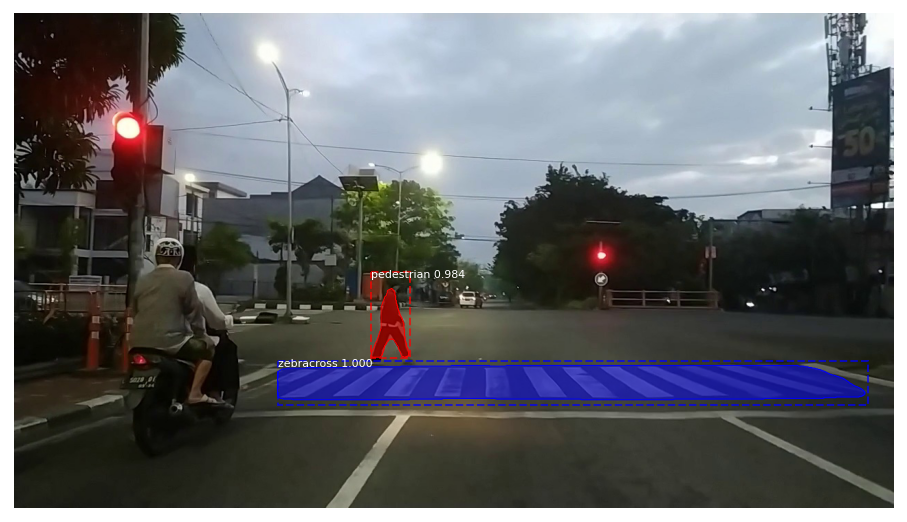
\includegraphics[scale=0.3]{gambar/hasil/resnet-50_fajar_800.png}
	\caption{Hasil Uji dari \textit{Backbone Resnet-50}}
	\label{fig:hasil-resnet50}
\end{figure}

\subsubsection{Hasil Pengujian dengan \textit{Backbone Resnet-101}}

Pada hasil pengujian dengan menggunakan satu gambar jalan raya pada pada saat pagi hari yang ditunjukkan pada gambar \ref{fig:hasil-resnet101}, didapatkan hasil skor yaitu :
\begin{enumerate}[nolistsep]
	\item Pejalan kaki (\textit{score} : 0,986)
	\item \textit{Zebracross} (\textit{score} : 0,995)
	\item Pengendara motor (\textit{score} : 0,999)
\end{enumerate}
Dari hasil tersebut, \textit{Backbone Resnet-101} dapat memprediksi gambar dengan benar, serta \textit{evaluation time} dari \textit{backbone} ini sebesar 0.961 detik
\begin{figure}[h] 
	\centering
	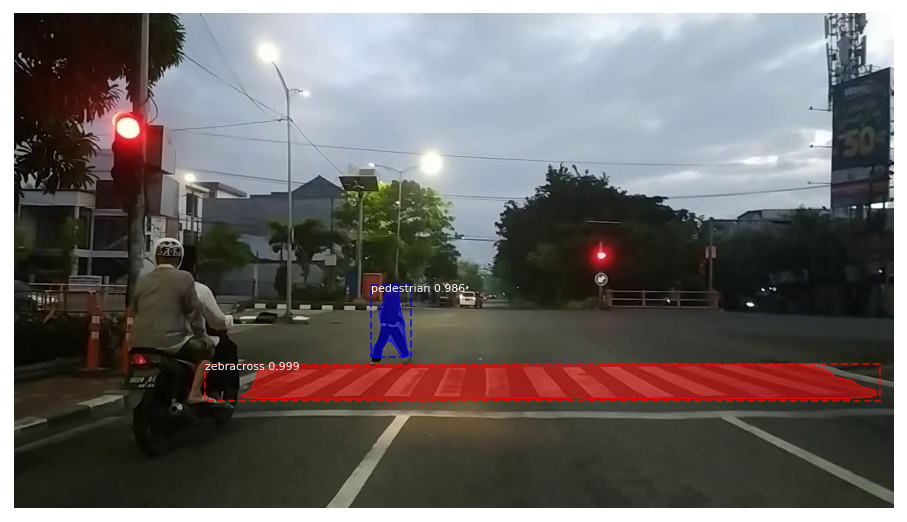
\includegraphics[scale=0.3]{gambar/hasil/resnet-101_fajar_800.png}
	\caption{Hasil Uji dari \textit{Backbone Resnet-101}}
	\label{fig:hasil-resnet101}
\end{figure}

\subsubsection{Hasil Pengujian dengan \textit{Backbone Mobilenet-V1}}

Pada hasil pengujian dengan menggunakan satu gambar jalan raya pada pada saat pagi hari yang ditunjukkan pada gambar \ref{fig:hasil-mobilenetv1}, didapatkan hasil skor yaitu :
\begin{enumerate}[nolistsep]
	\item Pejalan kaki (tidak terdeteksi)
	\item \textit{Zebracross} (terdeteksi 2  dengan \textit{score} : 0,942 dan 0.888)
	\item Pengendara motor (tidak terdeteksi)
\end{enumerate}
Dari hasil tersebut, \textit{Backbone Mobilenet-V1} tidak dapat memprediksi gambar dengan benar, serta \textit{evaluation time} dari \textit{backbone} ini sebesar 0.664 detik
\begin{figure}[h] 
	\centering
	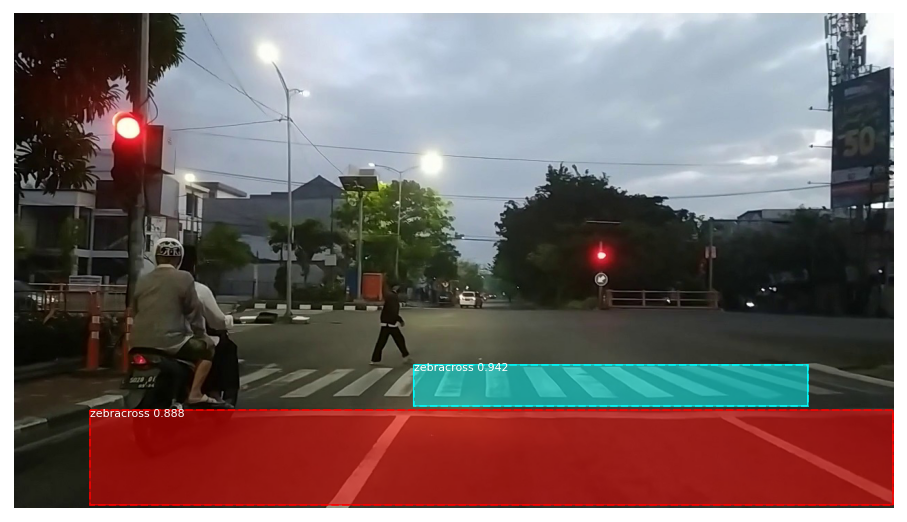
\includegraphics[scale=0.3]{gambar/fajar-frame800-mobilenetv1.png}
	\caption{Hasil Uji dari \textit{Backbone Mobilenet-V1}}
	\label{fig:hasil-mobilenetv1}
\end{figure}

Setelah melakukan \textit{testing} dengan menggunakan gambar pada \textit{testing set} pada keseluruhan model, maka tabel \ref{tab:result-comparasion} menunjukkan ringkasan dari perbandingan hasil \textit{testing} yang telah dilakukan. Parameter yang akan dibandingkan yaitu \textit{evaluation time} dan besar \textit{mean Average Precision}.

\begin{table}[h]
	\centering
	\caption{tabel Perbandingan Hasil \textit{Testing}}
	\resizebox{\textwidth}{!}{%
		\begin{tabular}{|c|l|r|r|}
			\hline
			\multicolumn{1}{|l|}{\textbf{No.}} & \textit{\textbf{Backbone}} & \textit{\textbf{Evaluation Time}} & \textbf{mAP} \\ \hline
			1                                  & ResNet-50                  & 0,763 s                           & 100\%        \\ \hline
			2                                  & ResNet-101                 & 0.961 s                             & 100\%        \\ \hline
			3                                  & MobileNet-v1               & 0.664 s                             & 25\%          \\ \hline
		\end{tabular}%
	}
	\label{tab:result-comparasion}
\end{table}

\section{Pengujian Perbedaan Waktu}
\label{sec:pengujian-waktu}

Pengujian pada perbedaan waktu bertujuan untuk mengetahui performa dan akurasi dari setiap model yang dihasilkan dengan waktu yang berbeda-beda (pagi, siang dan malam). \textit{File input} untuk pengujian ini terdapat 2 macam, yaitu gambar dengan format \textit{.jpg} dan video dengan format \textit{.mp4}.

\subsection{Pengujian di Pagi Hari}
\label{subsec:pagi}

Pada pengujian ini \textit{testing data} diambil dengan menggunakan kamera \textit{smartphone} yang menghasilkan video beresolusi 1280$\times$720 px berdurasi 63.43 s. Video tersebut mempunyai banyak \textit{frame} per detik sebanyak 30 fps serta total \textit{frame} yang dihasilkan sejumlah 1903 \textit{frame}. Gambar \ref{fig:comparasion-morning} merupakan perbandingan hasis deteksi dan segementasi dari ketiga \textit{backbone} yang digunakan pada waktu pagi hari.

\begin{figure}[h]
	\centering
	\begin{minipage}[b]{0.3\textwidth}
		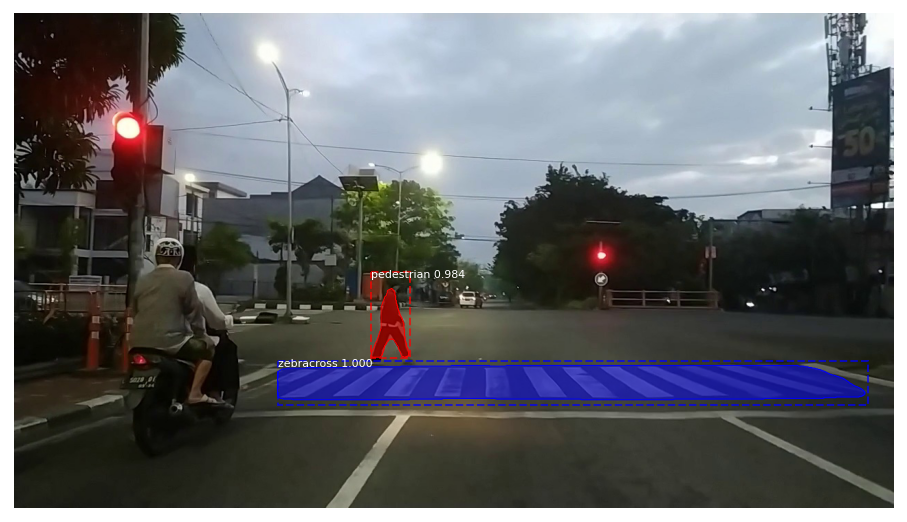
\includegraphics[width=\textwidth]{gambar/hasil/resnet-50_fajar_800.png}
		\caption*{(a) ResNet-50}
	\end{minipage}
	\hfill
	\begin{minipage}[b]{0.3\textwidth}
		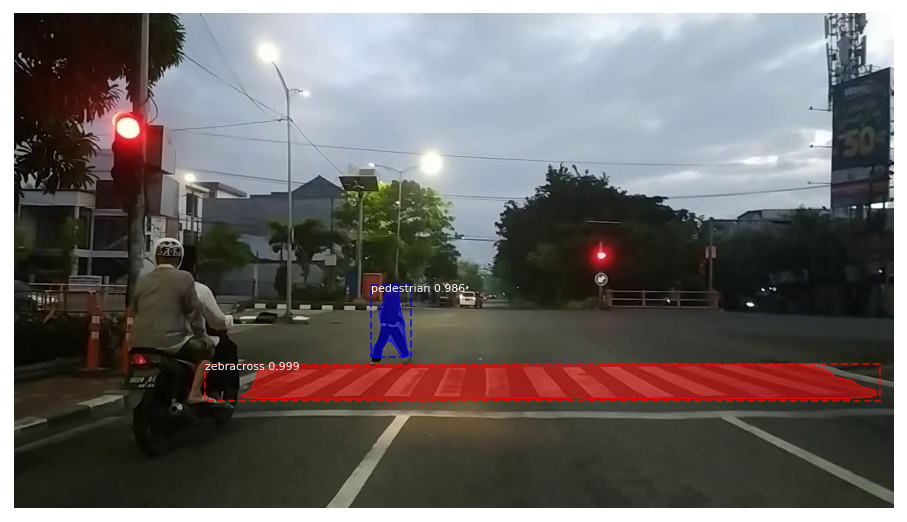
\includegraphics[width=\textwidth]{gambar/hasil/resnet-101_fajar_800.png}
		\caption*{(b) ResNet-101}
	\end{minipage}
	\hfill
	\begin{minipage}[b]{0.3\textwidth}
		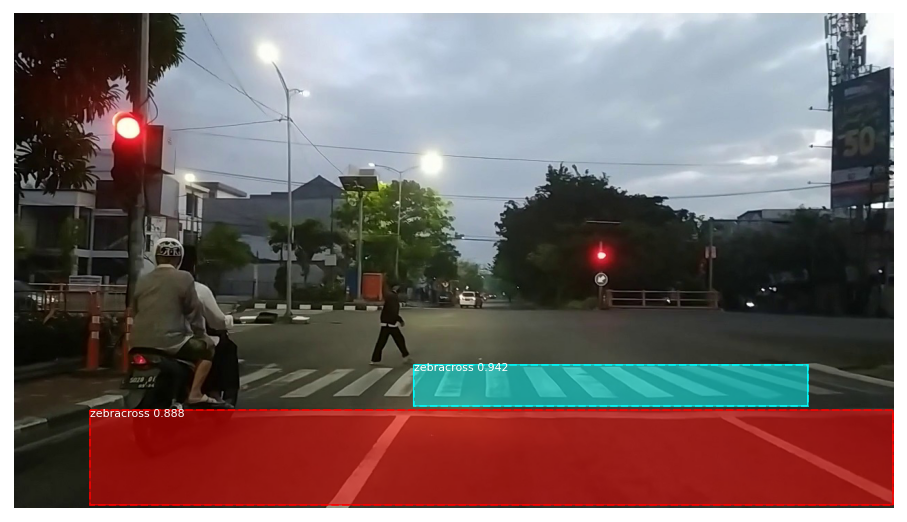
\includegraphics[width=\textwidth]{gambar/fajar-frame800-mobilenetv1.png}
		\caption*{(c) MobileNet-v1}
	\end{minipage}
	\caption{{Perbandingan Hasil pada Pagi Hari}}
	\label{fig:comparasion-morning}
\end{figure}

Untuk meguji performa model yang dihasilkan pada masing-masing \textit{backbone}, digunakan beberapa parameter nilai seperti \textit{precision, recall} dan \textit{F1-score} pada masing-masing kelas objek yang dideteksi. Perbandingan hasil evaluasi yang didapatkan masing-masing \textit{backbone} dapat dilihat pada Tabel \ref{tab:evaluate-morning}.

Pada Resnet-50 \textit{Average Precision} untuk semua kelas yang berhasil dideteksi adalah sebesar 100\% dan \textit{Average Recall} 100\% dengan \textit{testing time} selama 0,763 s. Sedangkan pada Resnet-101 memberikan hasil yang sama dengan Resnet-50 dengan \textit{AP} 100\% dan \textit{AR} 100\% dengan \textit{testing time} selama 0,961 s. Namun pada Mobilenet-v1 objek yang berhasil dideteksi hanya \textit{zebracross} (ditambah dengan \textit{background}), sehingga pada objek pejalan kaki dan pengendara motor mempunyai \textit{precision} bernilai 0\% serta \textit{Recall} dan \textit{F1-score} bernilai tidak terdefinisi atau \textit{NaN}. Hal ini dikarenakan nilai \textit{True Positif} pada pejalan kaki dan pengendara motor bernilai 0 (angka 0 dibagi nilai berapun memiliki hasil tidak terdefinisi). Nilai \textit{AP} yang dihasilkan pada evaluasi Mobilenet-v1 sebesar 37.5\% dengan \textit{testing time} selama 0.664 s.

\begin{table}[!h]
	\centering
	\caption{{Perbandingan Hasil Evaluasi pada Pagi Hari}}
	\begin{minipage}[b]{\textwidth}
		\centering
		\caption*{(a) ResNet-50}
		\begin{tabular}{|l|c|c|c|}
			\hline
			\multicolumn{1}{|c|}{\textbf{Kelas}} & \textit{\textbf{Precision (\%)}} & \textit{\textbf{Recall (\%)}} & \textit{\textbf{F1\_Score (\%)}} \\ \hline
			Background                           & 100                              & 100                           & 100                              \\ \hline
			Pedestrian                           & 100                              & 100                           & 100                              \\ \hline
			Zebracross                           & 100                              & 100                           & 100                              \\ \hline
			Motorbiker                           & 100                              & 100                           & 100                              \\ \hline
		\end{tabular}
	\end{minipage}
	\vfill
	\begin{minipage}[b]{\textwidth}
		\centering
		\caption*{(b) ResNet-101}
		\begin{tabular}{|l|c|c|c|}
			\hline
			\multicolumn{1}{|c|}{\textbf{Kelas}} & \textit{\textbf{Precision (\%)}} & \textit{\textbf{Recall (\%)}} & \textit{\textbf{F1\_Score (\%)}} \\ \hline
			Background                           & 100                              & 100                           & 100                              \\ \hline
			Pedestrian                           & 100                              & 100                           & 100                              \\ \hline
			Zebracross                           & 100                              & 100                           & 100                              \\ \hline
			Motorbiker                           & 100                              & 100                           & 100                              \\ \hline
		\end{tabular}
	\end{minipage}
	\vfill
	\begin{minipage}[b]{\textwidth}
		\centering
		\caption*{(c) MobileNet-v1}
		\begin{tabular}{|l|c|c|c|}
			\hline
			\multicolumn{1}{|c|}{\textbf{Kelas}} & \textit{\textbf{Precision (\%)}} & \textit{\textbf{Recall (\%)}} & \textit{\textbf{F1\_Score (\%)}} \\ \hline
			Background                           & 50                               & 33.33                         & 40                               \\ \hline
			Pedestrian                           & 0                                & NaN                           & NaN                              \\ \hline
			Zebracross                           & 100                              & 50                            & 66.66                            \\ \hline
			Motorbiker                           & 0                                & NaN                           & NaN                              \\ \hline
		\end{tabular}
	\end{minipage}
	\label{tab:evaluate-morning}
\end{table}

Selain menggunakan \textit{input data} berupa gambar, pada pengujian ini juga menggunakan \textit{input data} berupa \textit{file} video dengan format \textit{.mp4}. Proses \textit{testing} dibagi menjadi dua tahapan, tahap pertama memecah \textit{frame} video menjadi gambar dan melakukan prediksi serta tahap kedua menggabungkan kembali setiap \textit{frame} menjadi video. Tabel \ref{tab:video-morning} menunjukan waktu yang dibutuhkan untuk melakukan semua tahap prediksi pada \textit{file input} berbentuk video pada ketiga \textit{backbone}.

\begin{table}[!h]
	\centering{
		\caption{Waktu Prediksi pada \textit{File Input} Video dalam \textit{MM:SS}}
		\begin{tabular}{|l|c|c|c|c|}
			\hline
			\multicolumn{1}{|c|}{\textit{\textbf{Backbone}}} & \textit{\textbf{Tahap 1}} & \textit{\textbf{Tahap 2}} & \textit{\textbf{Total}} & \multicolumn{1}{l|}{\textit{\textbf{Output Size}}} 
			\\ \hline
			\textit{ResNet-50}                              & 07:24                     & 00:38                     & 08:03                   & 88.8 MB 
			\\ \hline
			\textit{ResNet-101}                                        & 07:54                     & 00:49                     & 08:44                   & 87.7 MB                                                                                       \\ \hline
			\textit{MobileNet-v1}                            & 06:50                     & 00:40                     & 07:31                   & 89.7 MB                                            \\ \hline
		\end{tabular}
	}
	\label{tab:video-morning}
\end{table}

\subsection{Pengujian di Siang Hari}
\label{subsec:siang}

Pada pengujian ini \textit{testing data} diambil dari video streaming \textit{youtube}\citep{test-siang} yang memiliki resolusi 1920$\times$1080 px berdurasi 29.4 s. Video tersebut mempunyai banyak \textit{frame} per detik sebanyak 25 fps serta total \textit{frame} yang dihasilkan sejumlah 735 \textit{frame}. Gambar \ref{fig:comparasion-afternoon} merupakan perbandingan hasis deteksi dan segementasi dari ketiga \textit{backbone} yang digunakan pada waktu siang hari.

\begin{figure}[!h]
	\centering
	\begin{minipage}[b]{0.3\textwidth}
		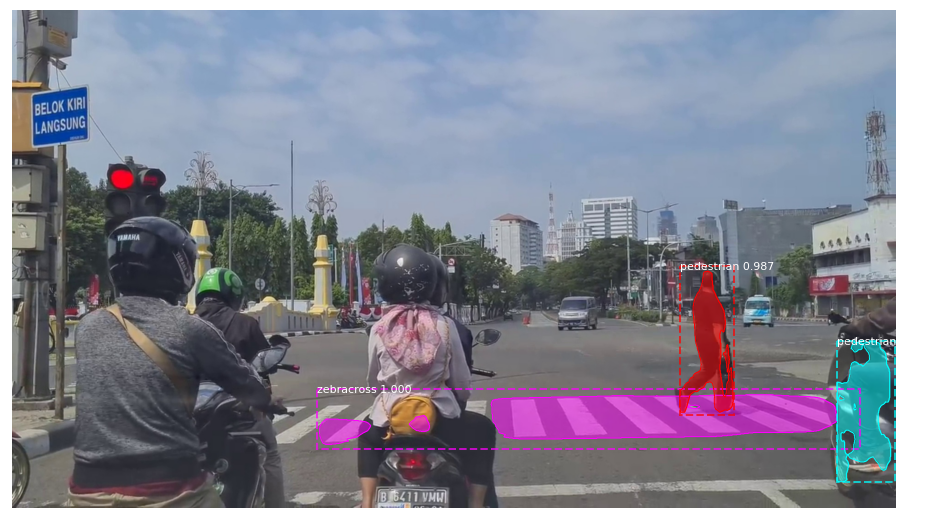
\includegraphics[width=\textwidth]{gambar/hasil/resnet-50_siang_465.png}
		\caption*{(a) ResNet-50}
	\end{minipage}
	\hfill
	\begin{minipage}[b]{0.3\textwidth}
		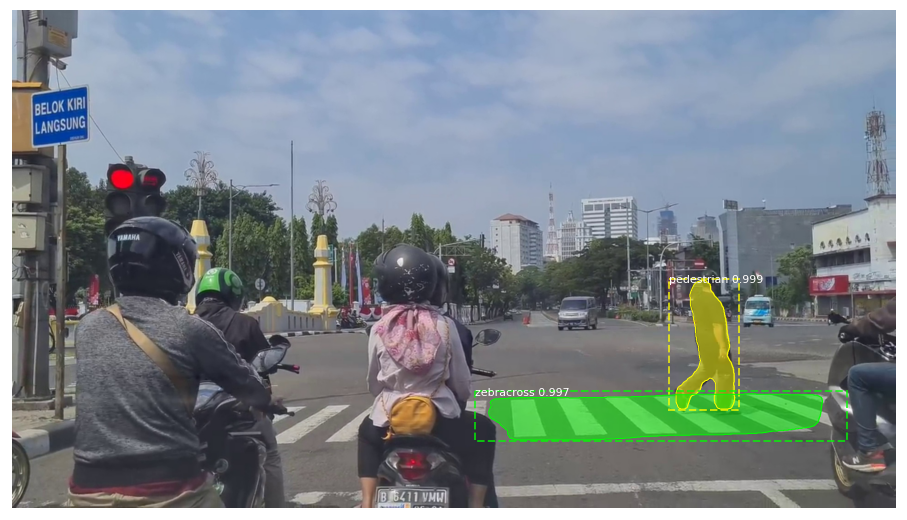
\includegraphics[width=\textwidth]{gambar/hasil/resnet-101_siang_465.png}
		\caption*{(b) ResNet-101}
	\end{minipage}
	\hfill
	\begin{minipage}[b]{0.3\textwidth}
		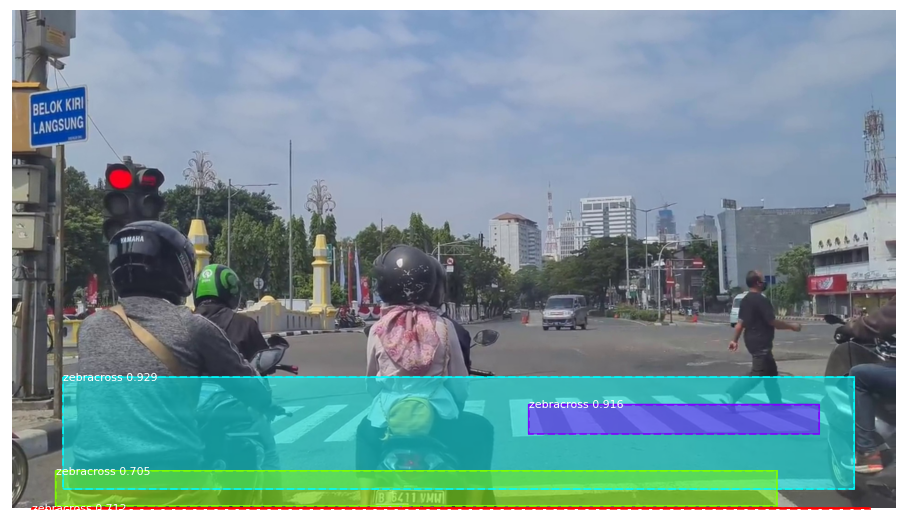
\includegraphics[width=\textwidth]{gambar/siang-frame465-mobilenetv1.png}
		\caption*{(c) MobileNet-v1}
	\end{minipage}
	\caption{{Perbandingan Hasil pada Siang Hari}}
	\label{fig:comparasion-afternoon}
\end{figure}

Perbandingan hasil evaluasi yang didapatkan masing-masing \textit{backbone} dengan membandingkan nilai \textit{precision, recall} dan \textit{F1-score} dapat dilihat pada Tabel \ref{tab:evaluate-afternoon}.

\begin{table}[!h]
	\centering
	\caption{{Perbandingan Hasil Evaluasi pada Siang Hari}}
	\begin{minipage}[b]{\textwidth}
		\centering
		\caption*{(a) ResNet-50}
		\begin{tabular}{|l|c|c|c|}
			\hline
			\multicolumn{1}{|c|}{\textbf{Kelas}} & \textit{\textbf{Precision (\%)}} & \textit{\textbf{Recall (\%)}} & \textit{\textbf{F1\_Score (\%)}} \\ \hline
			Background                           & 50                               & 25                            & 33.33                            \\ \hline
			Pedestrian                           & 100                              & 100                           & 100                              \\ \hline
			Zebracross                           & 50                               & 100                           & 66.66                            \\ \hline
			Motorbiker                           & 50                               & 66.66                         & 57.14                            \\ \hline
		\end{tabular}
	\end{minipage}
	\vfill
	\begin{minipage}[b]{\textwidth}
		\centering
		\caption*{(b) ResNet-101}
		\begin{tabular}{|l|c|c|c|}
			\hline
			\multicolumn{1}{|c|}{\textbf{Kelas}} & \textit{\textbf{Precision (\%)}} & \textit{\textbf{Recall (\%)}} & \textit{\textbf{F1\_Score (\%)}} \\ \hline
			Background                           & 100                              & 25                            & 40                               \\ \hline
			Pedestrian                           & 100                              & 100                           & 100                              \\ \hline
			Zebracross                           & 50                               & 100                           & 66.66                            \\ \hline
			Motorbiker                           & 50                               & 100                           & 66.66                            \\ \hline
		\end{tabular}
	\end{minipage}
	\vfill
	\begin{minipage}[b]{\textwidth}
		\centering
		\caption*{(c) MobileNet-v1}
		\begin{tabular}{|l|c|c|c|}
			\hline
			\multicolumn{1}{|c|}{\textbf{Kelas}} & \textit{\textbf{Precision (\%)}} & \textit{\textbf{Recall (\%)}} & \textit{\textbf{F1\_Score (\%)}} \\ \hline
			Background                           & 50                               & 14.28                         & 22.22                            \\ \hline
			Pedestrian                           & 0                                & NaN                           & NaN                              \\ \hline
			Zebracross                           & 50                               & 50                            & 50                               \\ \hline
			Motorbiker                           & 0                                & NaN                           & NaN                              \\ \hline
		\end{tabular}
	\end{minipage}
	\label{tab:evaluate-afternoon}
\end{table}

Pada Resnet-50 \textit{Average Precision} untuk semua kelas yang berhasil dideteksi adalah sebesar 62.5\% dan \textit{Average Recall} 72.915\% dengan \textit{testing time} selama 1,253 s. Sedangkan pada Resnet-101 memberikan hasil \textit{AP} sebesar 75\% dan \textit{AR} 81.5\% dengan \textit{testing time} selama 1,549 s. Namun pada Mobilenet-v1 objek yang berhasil dideteksi hanya \textit{zebra cross} (ditambah dengan \textit{background}) sama saat pengujian pada pagi hari. Nilai \textit{AP} yang dihasilkan pada evaluasi Mobilenet-v1 sebesar 25\% dengan \textit{testing time} selama 1,186 s.

Selain menggunakan \textit{input data} berupa gambar, pada pengujian ini juga menggunakan \textit{input data} berupa \textit{file} video dengan format \textit{.mp4}. Proses \textit{testing} dibagi menjadi dua tahapan, tahap pertama memecah \textit{frame} video menjadi gambar dan melakukan prediksi serta tahap kedua menggabungkan kembali setiap \textit{frame} menjadi video. Tabel \ref{tab:video-afternoon} menunjukan waktu total yang dibutuhkan untuk melakukan semua tahap prediksi pada \textit{file input} berbentuk video pada ketiga \textit{backbone}.

\begin{table}[!h]
	\centering{
		\caption{Waktu Prediksi pada \textit{File Input} Video dalam \textit{MM:SS}}
		\begin{tabular}{|l|c|c|c|c|}
			\hline
			\multicolumn{1}{|c|}{\textit{\textbf{Backbone}}} & \textit{\textbf{Tahap 1}} & \textit{\textbf{Tahap 2}} & \textit{\textbf{Total}} & \multicolumn{1}{l|}{\textit{\textbf{Output Size}}} \\ \hline
			\textit{ResNet-50}                              & 05:33                     & 00:30                     & 06:03                    & 52.8 MB                                            \\ \hline
			\textit{ResNet-101}                                        & 07:21                     & 00:36                     & 07:58                   & 50.1 MB                                           \\ \hline
			\textit{MobileNet-v1}                            & 04:03                     & 00:30                     & 04:33                   & 42 MB                                              \\ \hline
		\end{tabular}
	}
	\label{tab:video-afternoon}
\end{table}

\newpage

\subsection{Pengujian di Malam Hari}
\label{subsec:malam}

Pada pengujian ini \textit{testing data} diambil dari video \textit{streaming youtube} \citep{test-malam} yang memiliki resolusi 1920$\times$1080 px berdurasi 28.04 s. Video tersebut mempunyai banyak \textit{frame} per detik sebanyak 25 fps serta total \textit{frame} yang dihasilkan sejumlah 701 \textit{frame}. Gambar \ref{fig:comparasion-night} merupakan perbandingan hasis deteksi dan segementasi dari ketiga \textit{backbone} yang digunakan pada waktu siang hari.

\begin{figure}[H]
	\centering
	\begin{minipage}[b]{0.3\textwidth}
		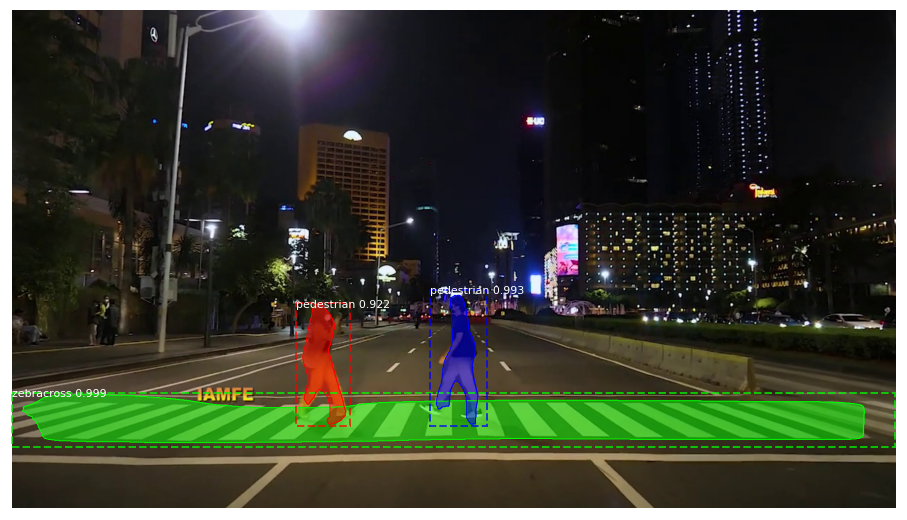
\includegraphics[width=\textwidth]{gambar/hasil/resnet-50_malam_180.png}
		\caption*{(a) ResNet-50}
	\end{minipage}
	\hfill
	\begin{minipage}[b]{0.3\textwidth}
		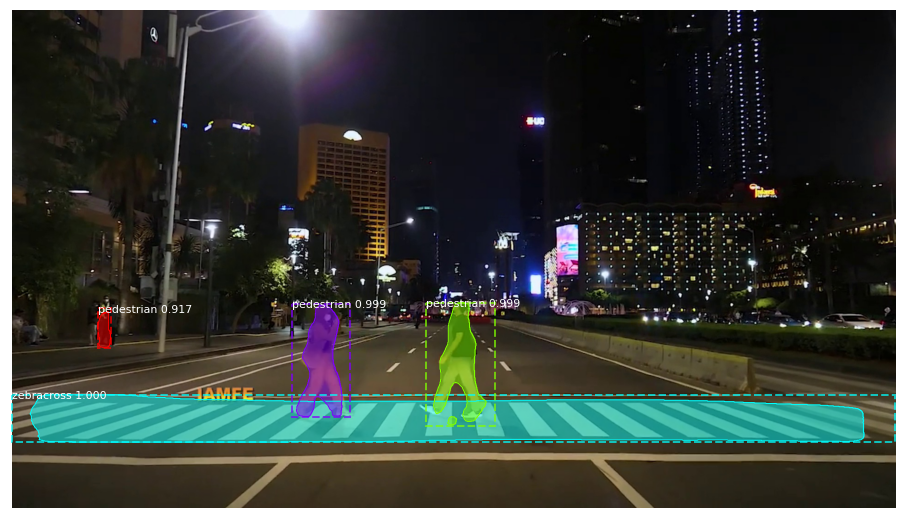
\includegraphics[width=\textwidth]{gambar/hasil/resnet-101_malam_180.png}
		\caption*{(b) ResNet-101}
	\end{minipage}
	\hfill
	\begin{minipage}[b]{0.3\textwidth}
		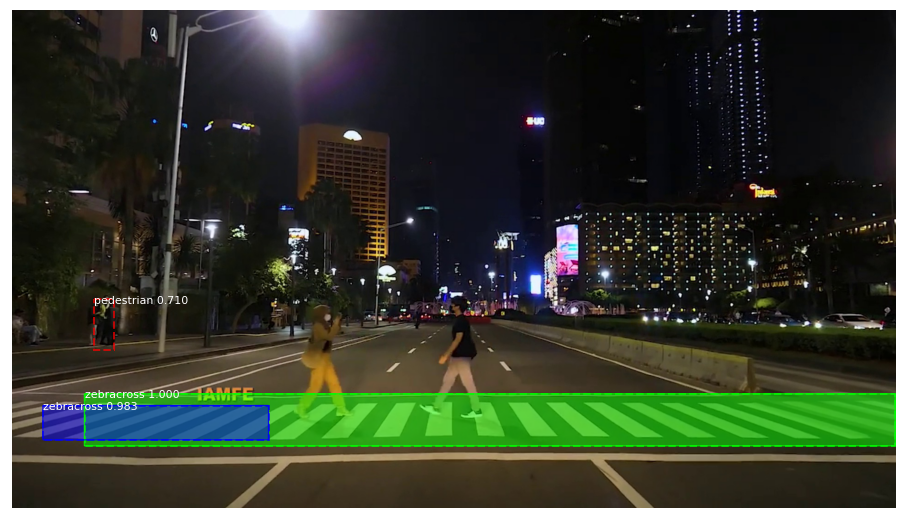
\includegraphics[width=\textwidth]{gambar/malam-frame180-mobilnetv1.png}
		\caption*{(c) MobileNet-v1}
	\end{minipage}
	\caption{{Perbandingan Hasil pada Malam Hari}}
	\label{fig:comparasion-night}
\end{figure}

Perbandingan hasil evaluasi yang didapatkan masing-masing \textit{backbone} dengan membandingkan nilai \textit{precision, recall} dan \textit{F1-score} dapat dilihat pada Tabel \ref{tab:evaluate-night}.

\begin{table}[H]
	\centering
	\caption{{Perbandingan Hasil Evaluasi pada Malam Hari}}
	\begin{minipage}[b]{\textwidth}
		\centering
		\caption*{(a) ResNet-50}
		\begin{tabular}{|l|c|c|c|}
			\hline
			\multicolumn{1}{|c|}{\textbf{Kelas}} & \textit{\textbf{Precision (\%)}} & \textit{\textbf{Recall (\%)}} & \textit{\textbf{F1\_Score (\%)}} \\ \hline
			Background                           & 100                              & 25                            & 40                               \\ \hline
			Pedestrian                           & 40                               & 100                           & 57.14                            \\ \hline
			Zebracross                           & 100                              & 100                           & 100                              \\ \hline
			Motorbiker                           & -                                & -                             & -                                \\ \hline
		\end{tabular}	
		
	\end{minipage}
	\vfill
	\begin{minipage}[b]{\textwidth}
		\centering
		\caption*{(b) ResNet-101}
		\begin{tabular}{|l|c|c|c|}
			\hline
			\multicolumn{1}{|c|}{\textbf{Kelas}} & \textit{\textbf{Precision (\%)}} & \textit{\textbf{Recall (\%)}} & \textit{\textbf{F1\_Score (\%)}} \\ \hline
			Background                           & 100                              & 33.33                         & 50                               \\ \hline
			Pedestrian                           & 60                               & 100                           & 74.9                             \\ \hline
			Zebracross                           & 100                              & 100                           & 100                              \\ \hline
			Motorbiker                           & -                                & -                             & -                                \\ \hline
		\end{tabular}
		
	\end{minipage}
	\vfill
	\begin{minipage}[b]{\textwidth}
		\centering
		\caption*{(c) MobileNet-v1}
		\begin{tabular}{|l|c|c|c|}
			\hline
			\multicolumn{1}{|c|}{\textbf{Kelas}} & \textit{\textbf{Precision (\%)}} & \textit{\textbf{Recall (\%)}} & \textit{\textbf{F1\_Score (\%)}} \\ \hline
			Background                           & 50                               & 16.66                         & 25                               \\ \hline
			Pedestrian                           & 0                                & NaN                           & NaN                              \\ \hline
			Zebracross                           & 100                              & 50                            & 66.66                            \\ \hline
			Motorbiker                           & -                                & -                             & -                                \\ \hline
		\end{tabular}
		
	\end{minipage}
	
	\label{tab:evaluate-night}
\end{table}

Pada gambar yang diuji untuk malam hari hanya memiliki 3 kelas saja yaitu \textit{background}, pejalan kaki serta \textit{zebracross} tanpa adanya pengendara motor. Resnet-50 mempunyai nilai \textit{Average Precision} untuk semua kelas yang berhasil dideteksi adalah sebesar 80\% dan \textit{Average Recall} 75\% dengan \textit{testing time} selama 1,069 s. Sedangkan pada Resnet-101 memberikan hasil \textit{AP} sebesar 86.67\% dan \textit{AR} 77.77\% dengan \textit{testing time} selama 1,215 s. Namun pada Mobilenet-v1 objek yang berhasil dideteksi hanya \textit{zebracross} (ditambah dengan \textit{background}) sama saat pengujian pada pagi dan siang hari. Nilai \textit{AP} yang dihasilkan pada evaluasi Mobilenet-v1 sebesar 50\% dengan \textit{testing time} selama 1,051 s.

Selain menggunakan \textit{input data} berupa gambar, pada pengujian ini juga menggunakan \textit{input data} berupa \textit{file} video dengan format \textit{.mp4}. Proses \textit{testing} dibagi menjadi dua tahapan, tahap pertama memecah \textit{frame} video menjadi gambar dan melakukan prediksi serta tahap kedua menggabungkan kembali setiap \textit{frame} menjadi video. Tabel \ref{tab:video-night} menunjukan waktu yang dibutuhkan untuk melakukan semua tahap prediksi pada \textit{file input} berbentuk video pada ketiga \textit{backbone}.

\begin{table}[H]
	\centering{
		\caption{Waktu Prediksi pada \textit{File Input} Video dalam \textit{MM:SS}}
		\begin{tabular}{|l|c|c|c|l|}
			\hline
			\multicolumn{1}{|c|}{\textit{\textbf{Backbone}}} & \textit{\textbf{Tahap 1}} & \textit{\textbf{Tahap 2}} & \textit{\textbf{Total}} & \textit{\textbf{Output Size}} \\ \hline
			\textit{ResNet-50}                              & 04:23                     & 00:28                     & 04:51                     & 38.7 MB                     \\ \hline
			\textit{ResNet-101}                                        & 04:49                     & 00:34                     & 05:23                   & 39.1 MB                       \\ \hline
			\textit{MobileNet-v1}                            & 03:39                     & 00:28                     & 04:07                   & 36.1 MB                       \\ \hline
		\end{tabular}
	}
	\label{tab:video-night}
\end{table}


\subsection{Perbandingan Hasil Evaluasi pada Perbedaan Waktu}
\label{subsec:compare-eval}

Setelah membandingkan hasil evaluasi model setiap perbedaan waktu, pada bagian ini akan dibandingkan peforma setiap model untuk keseluruhan perbedaan waktu (pagi, siang dan malam hari). 

\subsubsection{ResNet-50}

Pada proses evaluasi model dengan menggunakan seluruh \textit{testing data} (pagi, siang dan malam hari) didapatkan beberapa hasil skor yaitu :
\begin{enumerate}[nolistsep]
	\item \textit{mean Average Precision(mAP)} : 66.785\%
	\item \textit{mean Average Recall(mAR)} : 77\%
	\item \textit{F1-score} : 71.529\%
\end{enumerate}
Hasil tersebut didapatkan setelah dilakukan proses pencarian nilai \textit{Trur Positif, False Positif} dan \textit{False Negatif} seperti yang ditunjukkan pada \textit{confusion matrix} pada Gambar \ref{fig:confmatrix-resnet50}.

\begin{figure}[H]
	\centering
	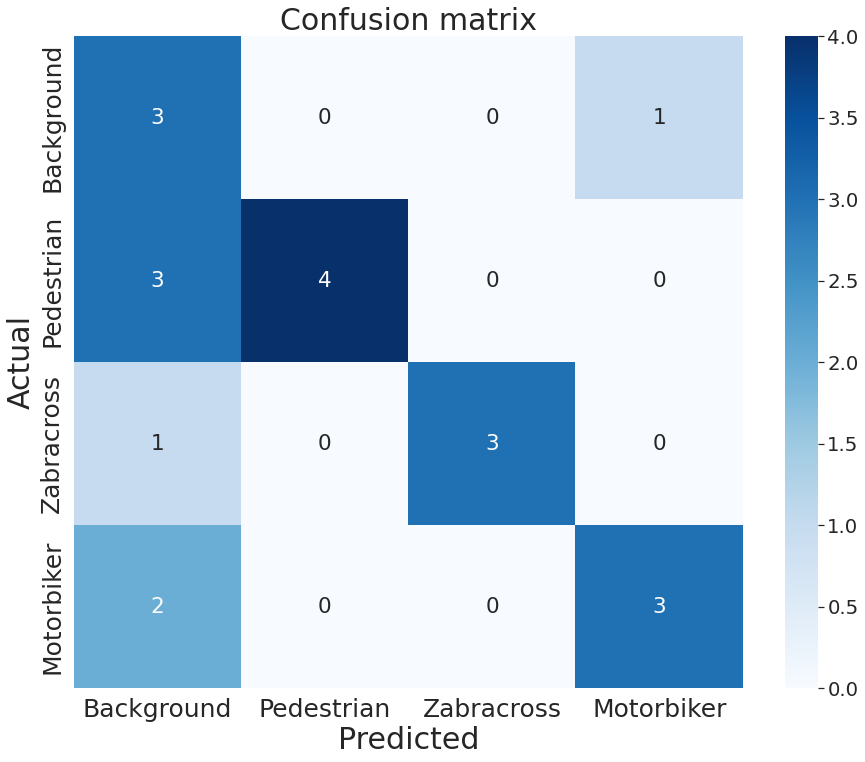
\includegraphics[scale=0.3]{gambar/confmatrix/all-resnet50-blue.png}
	\caption{\textit{Confusion Matrix} ResNet-50}
	\label{fig:confmatrix-resnet50}
\end{figure}

\subsubsection{ResNet-101}

Pada proses evaluasi model dengan menggunakan seluruh \textit{testing data} (pagi, siang dan malam hari) didapatkan beberapa hasil skor yaitu :
\begin{enumerate}[nolistsep]
	\item \textit{mean Average Precision(mAP)} : 76.605\%
	\item \textit{mean Average Recall(mAR)} : 85.375\%
	\item \textit{F1-score} : 80.302\%
\end{enumerate}
Hasil tersebut didapatkan setelah dilakukan proses pencarian nilai \textit{Trur Positif, False Positif} dan \textit{False Negatif} seperti yang ditunjukkan pada \textit{confusion matrix} pada Gambar \ref{fig:confmatrix-resnet101}.

\begin{figure}[H]
	\centering
	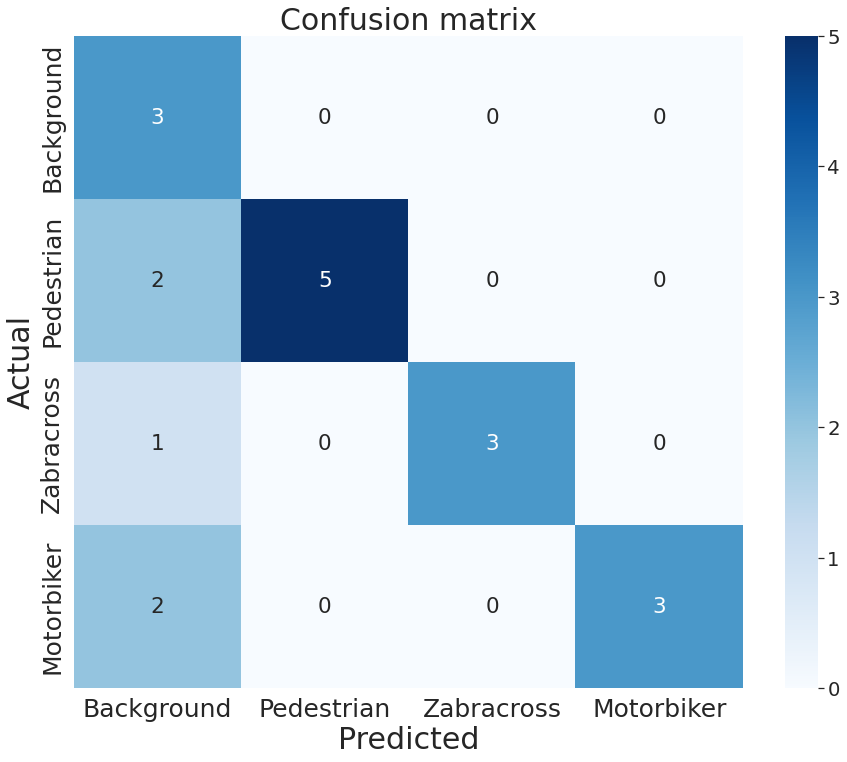
\includegraphics[scale=0.3]{gambar/confmatrix/all-resnet101-blue.png}
	\caption{\textit{Confusion Matrix} ResNet-101}
	\label{fig:confmatrix-resnet101}
\end{figure}

\subsubsection{MobileNet-v1}

Pada proses evaluasi model dengan menggunakan seluruh \textit{testing data} (pagi, siang dan malam hari) didapatkan beberapa hasil skor yaitu :
\begin{enumerate}[nolistsep]
	\item \textit{mean Average Precision(mAP)} : 25\%
	\item \textit{mean Average Recall(mAR)} : \textit{NaN}
	\item \textit{F1-score} : \textit{NaN}
\end{enumerate}
Hasil tersebut didapatkan setelah dilakukan proses pencarian nilai \textit{Trur Positif, False Positif} dan \textit{False Negatif} seperti yang ditunjukkan pada \textit{confusion matrix} pada Gambar \ref{fig:confmatrix-mobilenetv1}.

\begin{figure}[H]
	\centering
	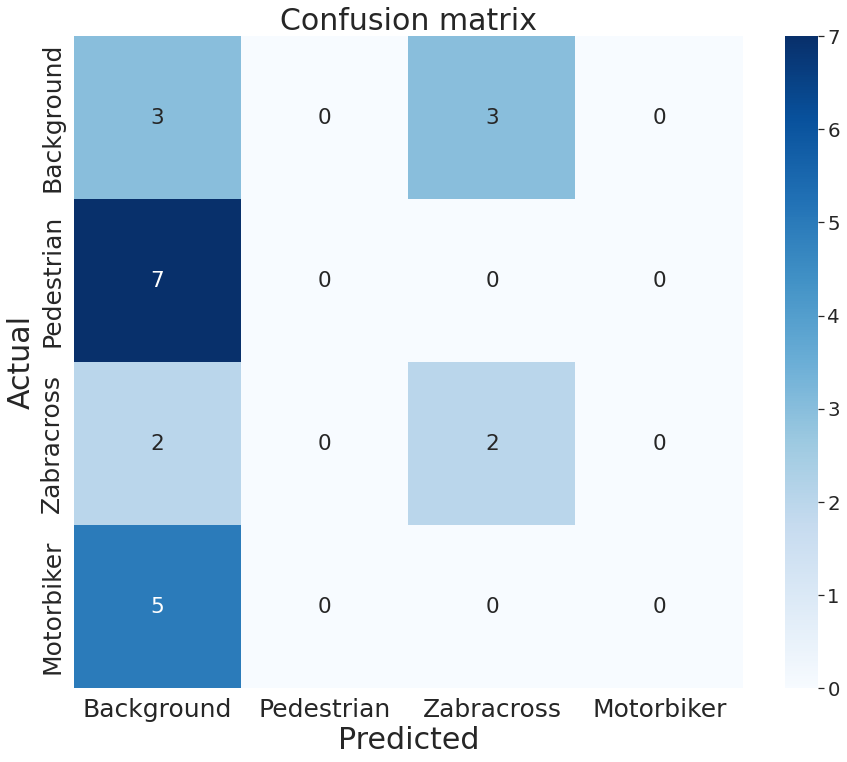
\includegraphics[scale=0.3]{gambar/confmatrix/all-mobilenetv1-blue.png}
	\caption{\textit{Confusion Matrix} MobileNet-v1}
	\label{fig:confmatrix-mobilenetv1}
\end{figure}